% Editable native annotations around unchanged verified IDE photographs.
\par
\begin{figure}[htbp]
  \centering
  \sbox0{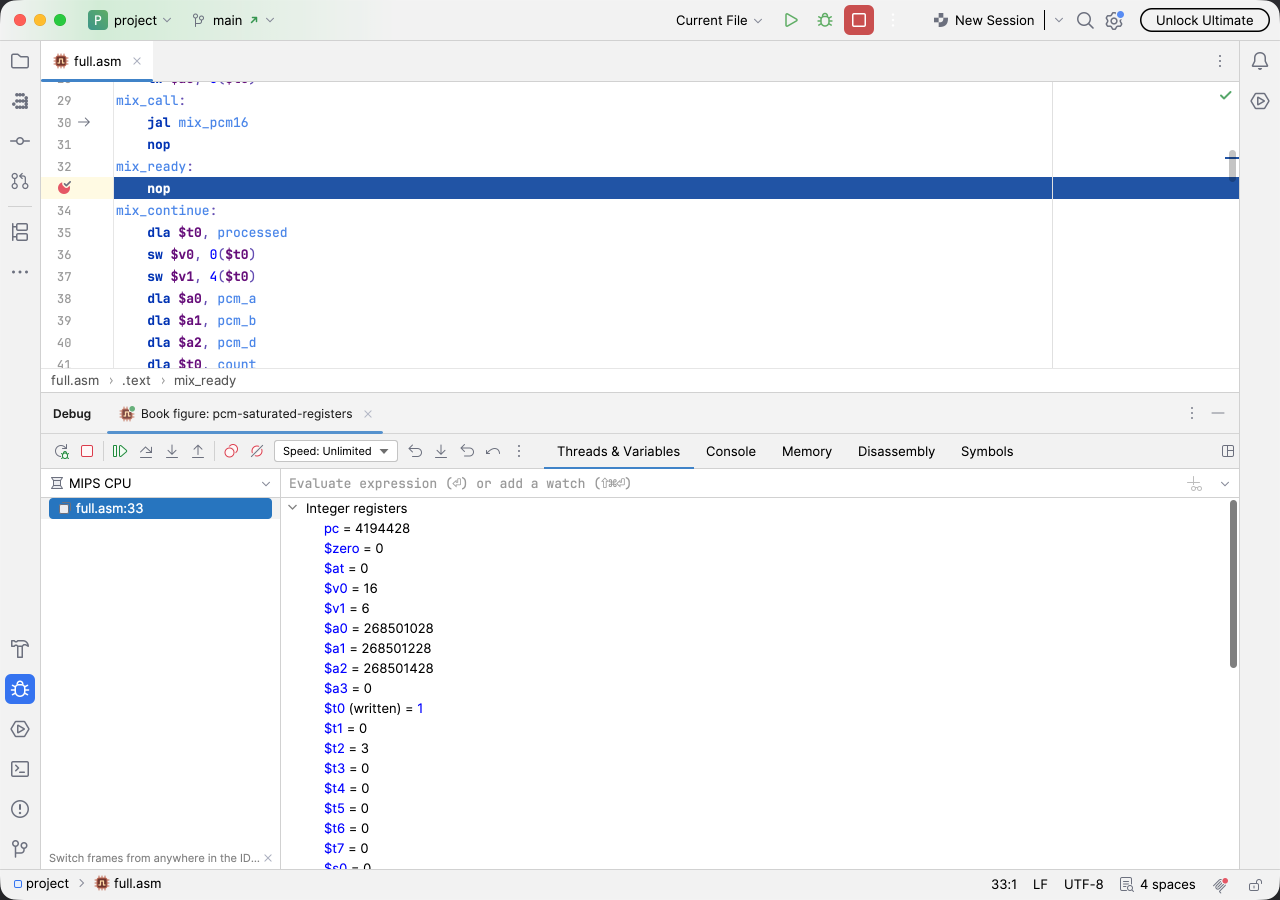
\includegraphics[artifact]{book/captures/020-pcm-mixing/f01/registers.png}}
  \sbox2{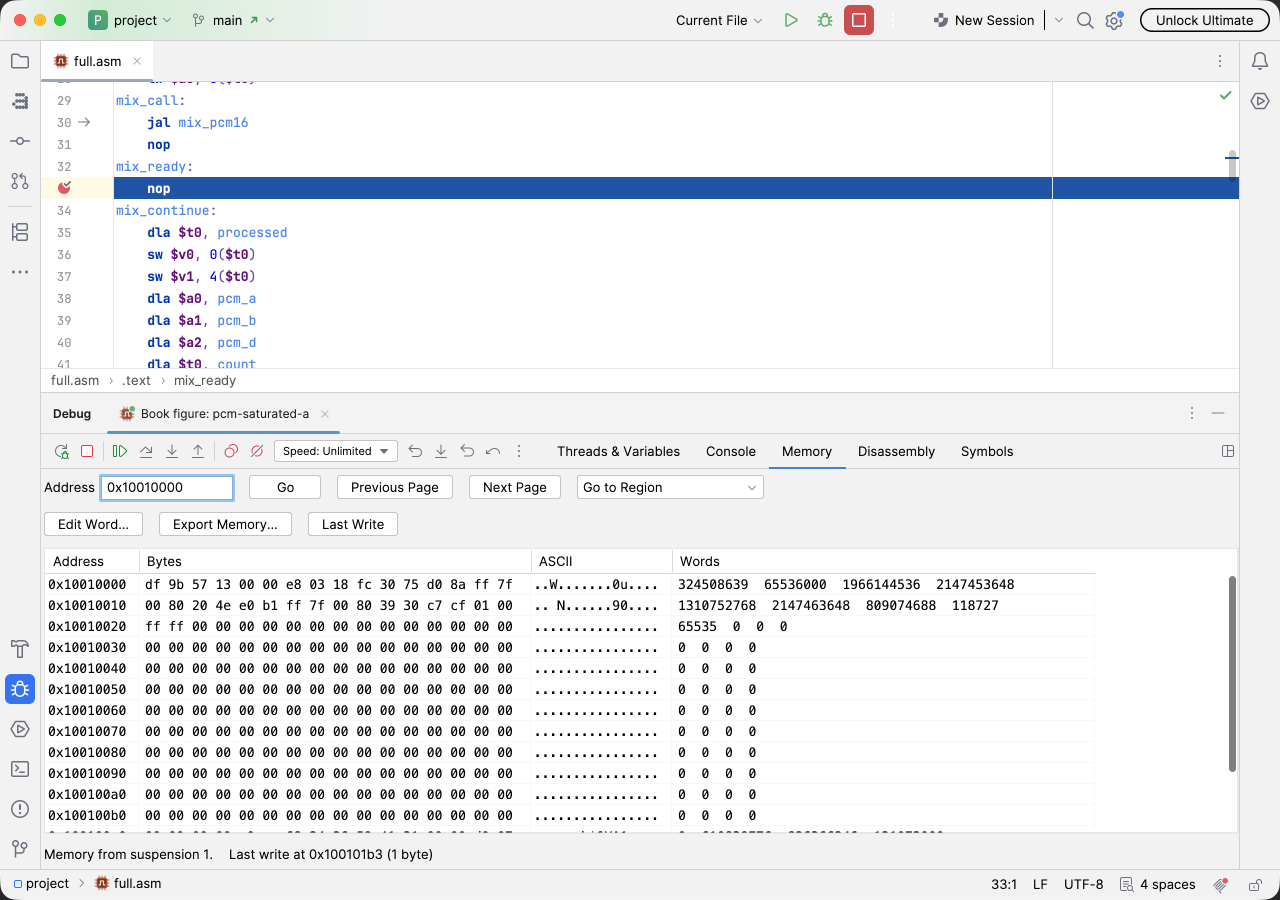
\includegraphics[artifact]{book/captures/020-pcm-mixing/f01/a.png}}
  \sbox4{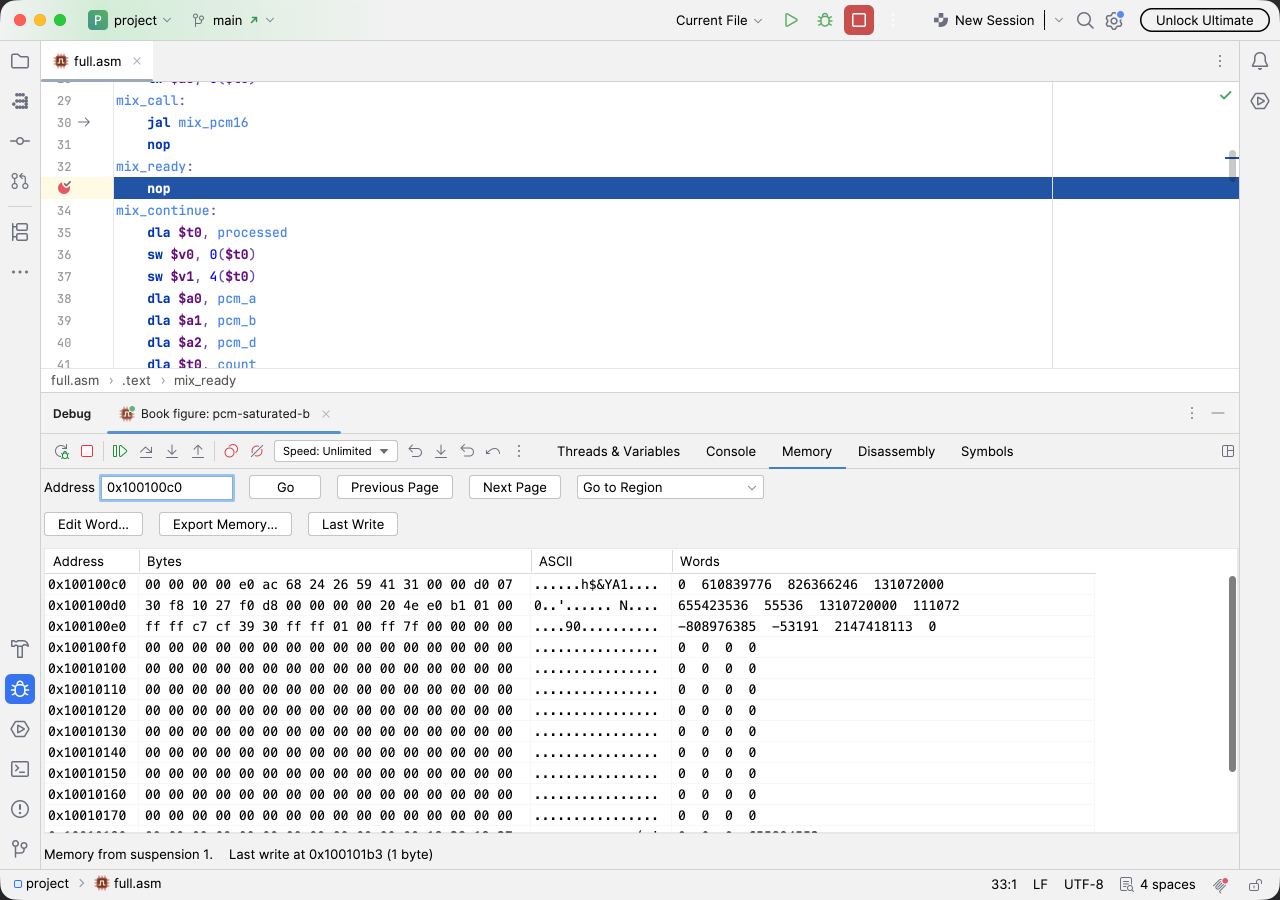
\includegraphics[artifact]{book/captures/020-pcm-mixing/f01/b.png}}
  \sbox6{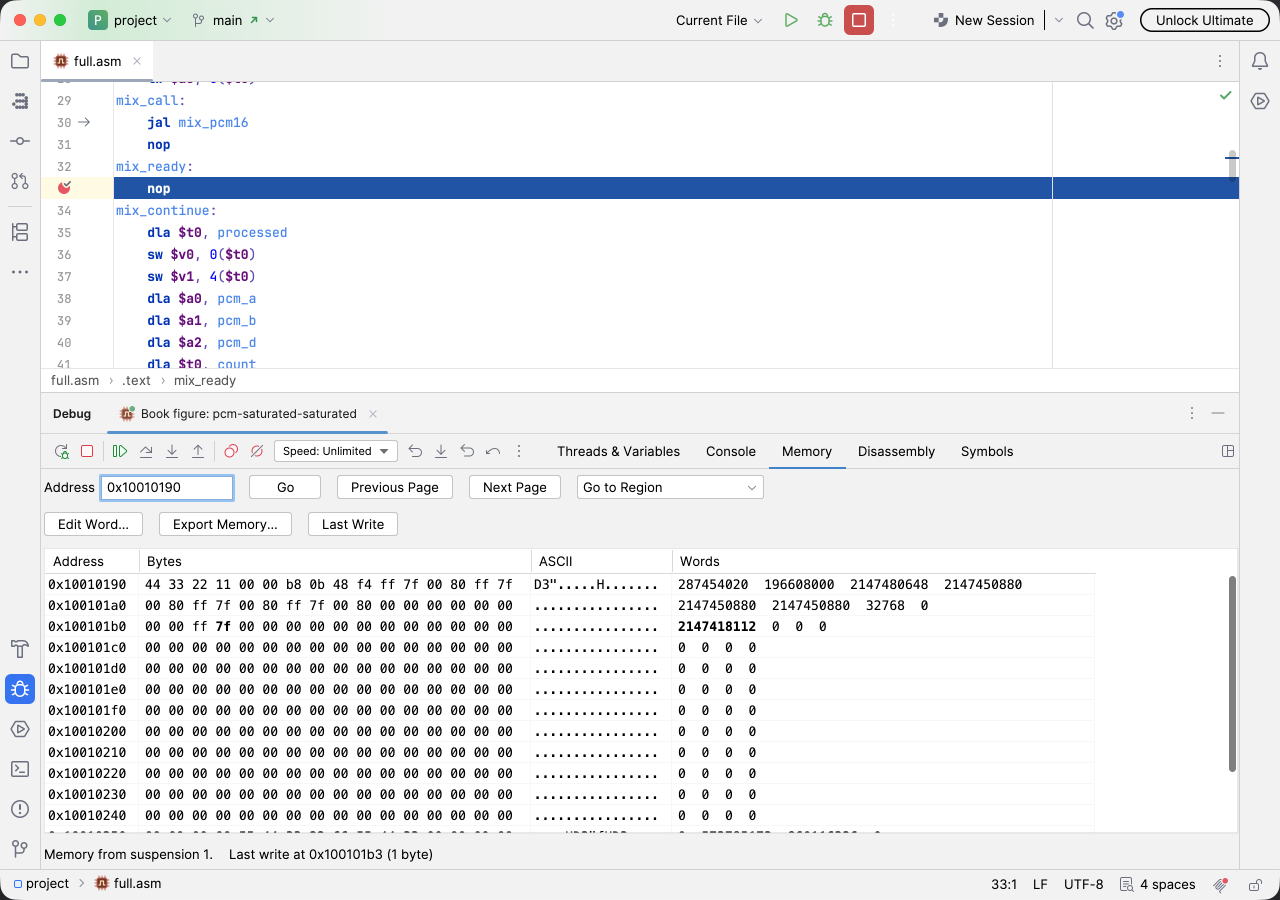
\includegraphics[artifact]{book/captures/020-pcm-mixing/f01/saturated.png}}
  \sbox8{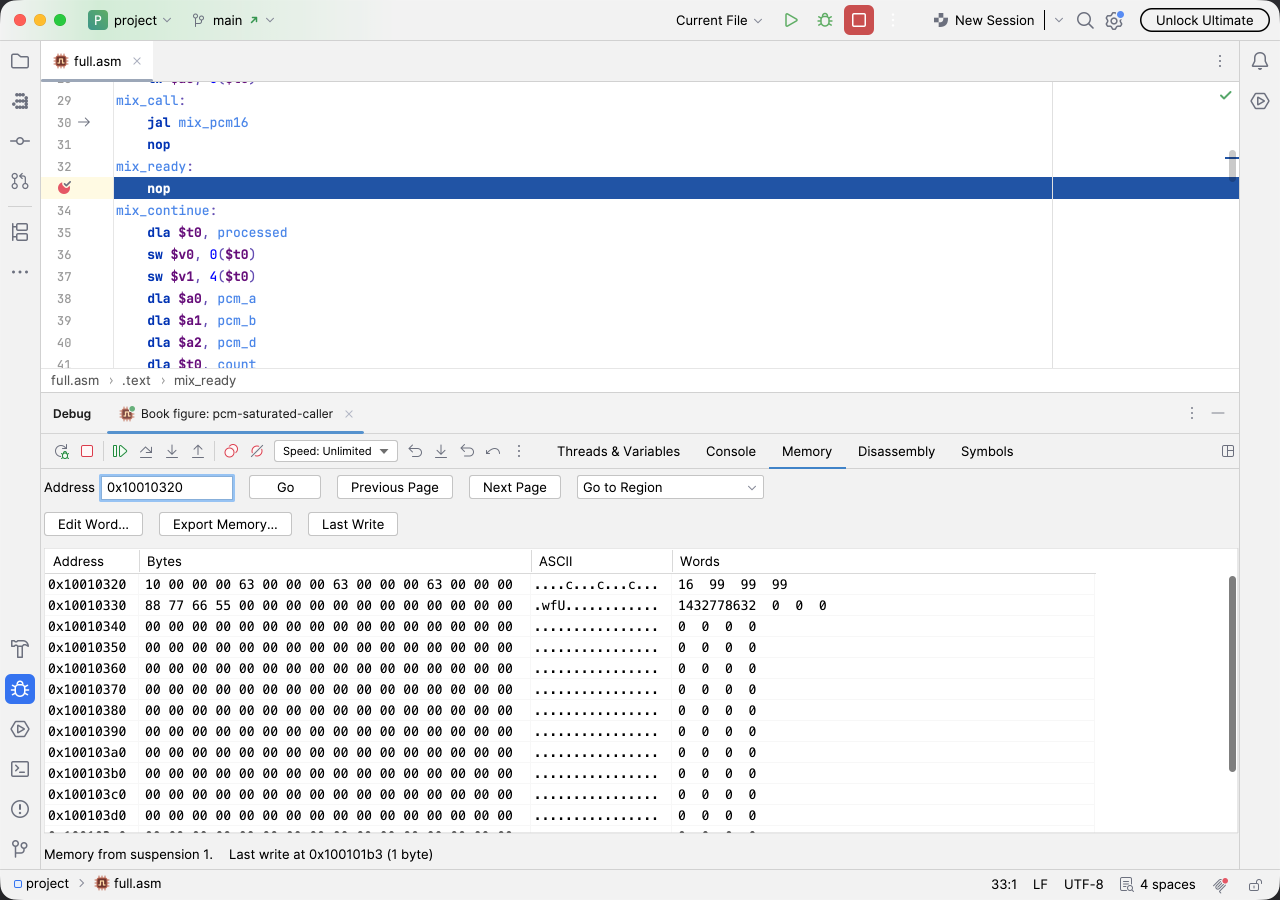
\includegraphics[artifact]{book/captures/020-pcm-mixing/f01/caller.png}}
  \edef\MARSpcmsaturatedsourceLeft{\the\dimexpr0.036718750\wd0\relax}
  \edef\MARSpcmsaturatedsourceBottom{\the\dimexpr0.774444444\ht0\relax}
  \edef\MARSpcmsaturatedsourceRight{\the\dimexpr0.713281250\wd0\relax}
  \edef\MARSpcmsaturatedsourceTop{\the\dimexpr0.170000000\ht0\relax}
  \edef\MARSpcmsaturatedregistersLeft{\the\dimexpr0.246093750\wd0\relax}
  \edef\MARSpcmsaturatedregistersBottom{\the\dimexpr0.312222222\ht0\relax}
  \edef\MARSpcmsaturatedregistersRight{\the\dimexpr0.553906250\wd0\relax}
  \edef\MARSpcmsaturatedregistersTop{\the\dimexpr0.640000000\ht0\relax}
  \edef\MARSpcmsaturatedaLeft{\the\dimexpr0.034375000\wd2\relax}
  \edef\MARSpcmsaturatedaBottom{\the\dimexpr0.311111111\ht2\relax}
  \edef\MARSpcmsaturatedaRight{\the\dimexpr0.584375000\wd2\relax}
  \edef\MARSpcmsaturatedaTop{\the\dimexpr0.608888889\ht2\relax}
  \edef\MARSpcmsaturatedbLeft{\the\dimexpr0.034375000\wd4\relax}
  \edef\MARSpcmsaturatedbBottom{\the\dimexpr0.311111111\ht4\relax}
  \edef\MARSpcmsaturatedbRight{\the\dimexpr0.584375000\wd4\relax}
  \edef\MARSpcmsaturatedbTop{\the\dimexpr0.608888889\ht4\relax}
  \edef\MARSpcmsaturatedsaturatedLeft{\the\dimexpr0.034375000\wd6\relax}
  \edef\MARSpcmsaturatedsaturatedBottom{\the\dimexpr0.311111111\ht6\relax}
  \edef\MARSpcmsaturatedsaturatedRight{\the\dimexpr0.584375000\wd6\relax}
  \edef\MARSpcmsaturatedsaturatedTop{\the\dimexpr0.608888889\ht6\relax}
  \edef\MARSpcmsaturatedcallerLeft{\the\dimexpr0.034375000\wd8\relax}
  \edef\MARSpcmsaturatedcallerBottom{\the\dimexpr0.334444444\ht8\relax}
  \edef\MARSpcmsaturatedcallerRight{\the\dimexpr0.584375000\wd8\relax}
  \edef\MARSpcmsaturatedcallerTop{\the\dimexpr0.608888889\ht8\relax}
  \begin{tikzpicture}[alt={Six annotated panels at mix_ready show returns sixteen and six, unchanged input halfwords, saturated output and caller words sixteen,99,99,99. Exact sums positive 40000 and negative 40000 become 32767 and minus 32768. Exact endpoint sums remain unchanged and do not count as clipping. Wrapping output is still zero.}]
    \node[anchor=north west,inner sep=0,font=\small\bfseries] (source-title) at (6mm,0) {Next instruction at this boundary};
    \node[anchor=north west,inner sep=0] (source) at ([yshift=-1mm]source-title.south west) {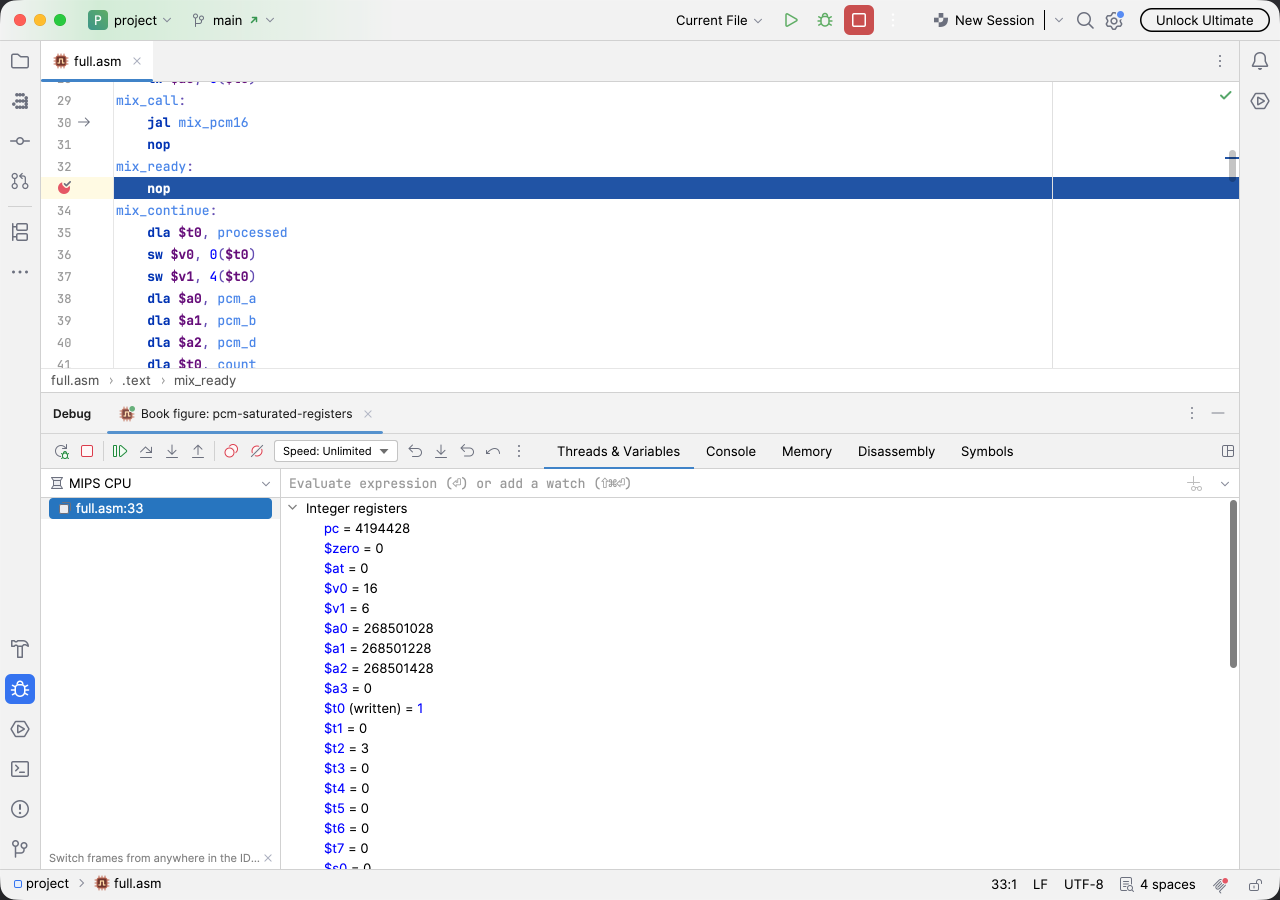
\includegraphics[width=0.54\linewidth,artifact,trim={\MARSpcmsaturatedsourceLeft{} \MARSpcmsaturatedsourceBottom{} \MARSpcmsaturatedsourceRight{} \MARSpcmsaturatedsourceTop{}},clip]{book/captures/020-pcm-mixing/f01/registers.png}};
    \begin{scope}[shift={(source.south west)},x={($(source.south east)-(source.south west)$)},y={($(source.north west)-(source.south west)$)}]
      \draw[black,line width=0.7pt] (0.215625000,0.080000000) rectangle (0.384375000,0.520000000);
      \node[draw=black,fill=white,circle,inner sep=1.5pt,font=\footnotesize] at ($(0.215625000,0.520000000)+(-3mm,0)$) {1};
    \end{scope}
    \node[anchor=north west,inner sep=0,font=\small\bfseries] (registers-title) at (0.58\linewidth,0 |- source-title.north) {Current return values};
    \node[anchor=north west,inner sep=0] (registers) at ([yshift=-1mm]registers-title.south west) {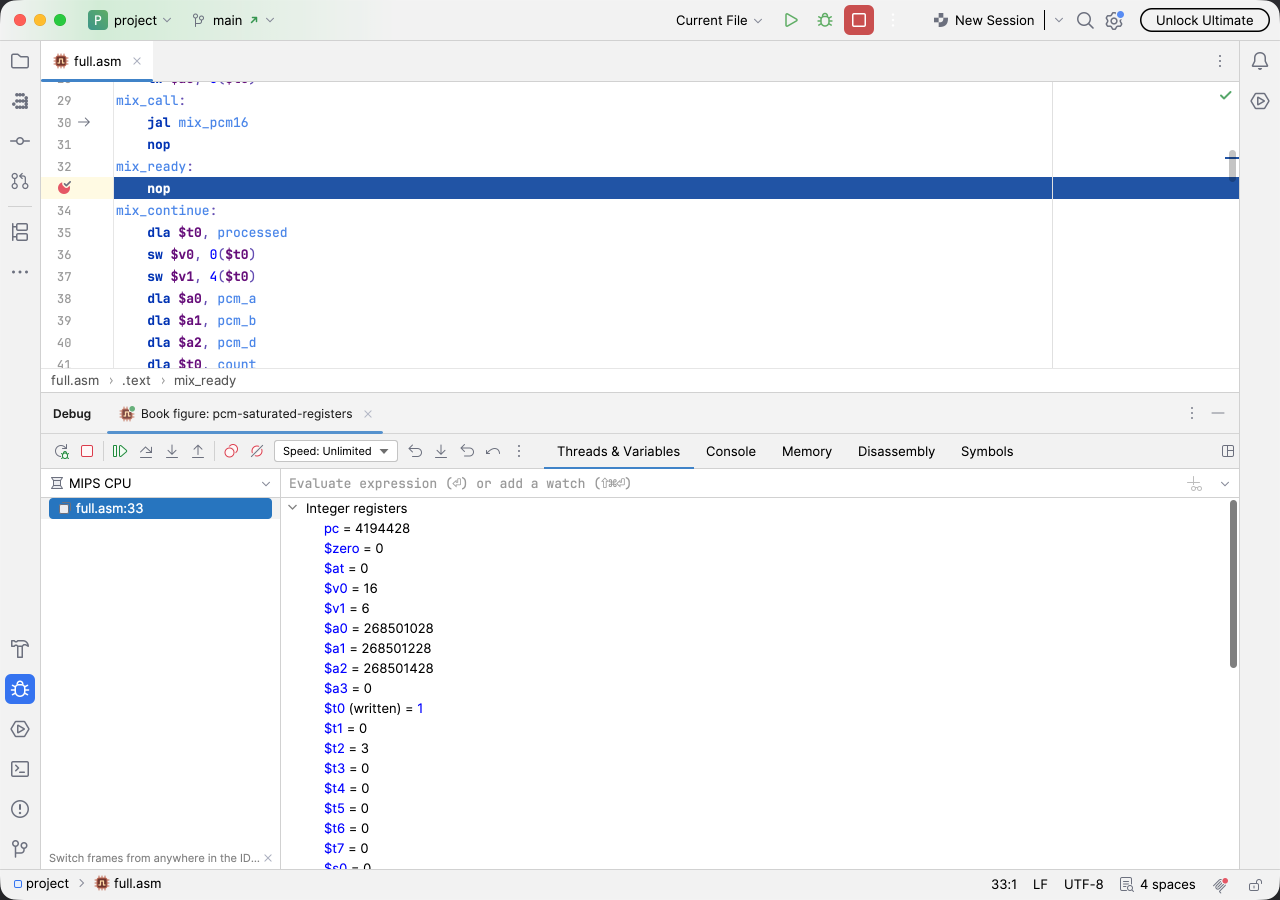
\includegraphics[width=0.42\linewidth,artifact,trim={\MARSpcmsaturatedregistersLeft{} \MARSpcmsaturatedregistersBottom{} \MARSpcmsaturatedregistersRight{} \MARSpcmsaturatedregistersTop{}},clip]{book/captures/020-pcm-mixing/f01/registers.png}};
    \begin{scope}[shift={(registers.south west)},x={($(registers.south east)-(registers.south west)$)},y={($(registers.north west)-(registers.south west)$)}]
      \draw[black,line width=0.7pt] (0.023437500,0.023255814) rectangle (0.250000000,0.953488372);
      \node[draw=black,fill=white,circle,inner sep=1.5pt,font=\footnotesize] at ($(0.023437500,0.953488372)+(-3mm,0)$) {2};
    \end{scope}
    \node[anchor=north west,inner sep=0,font=\small\bfseries] (a-title) at ([yshift=-1mm]source.south west) {Input A: signed halfwords};
    \node[anchor=north west,inner sep=0] (a) at ([yshift=-1mm]a-title.south west) {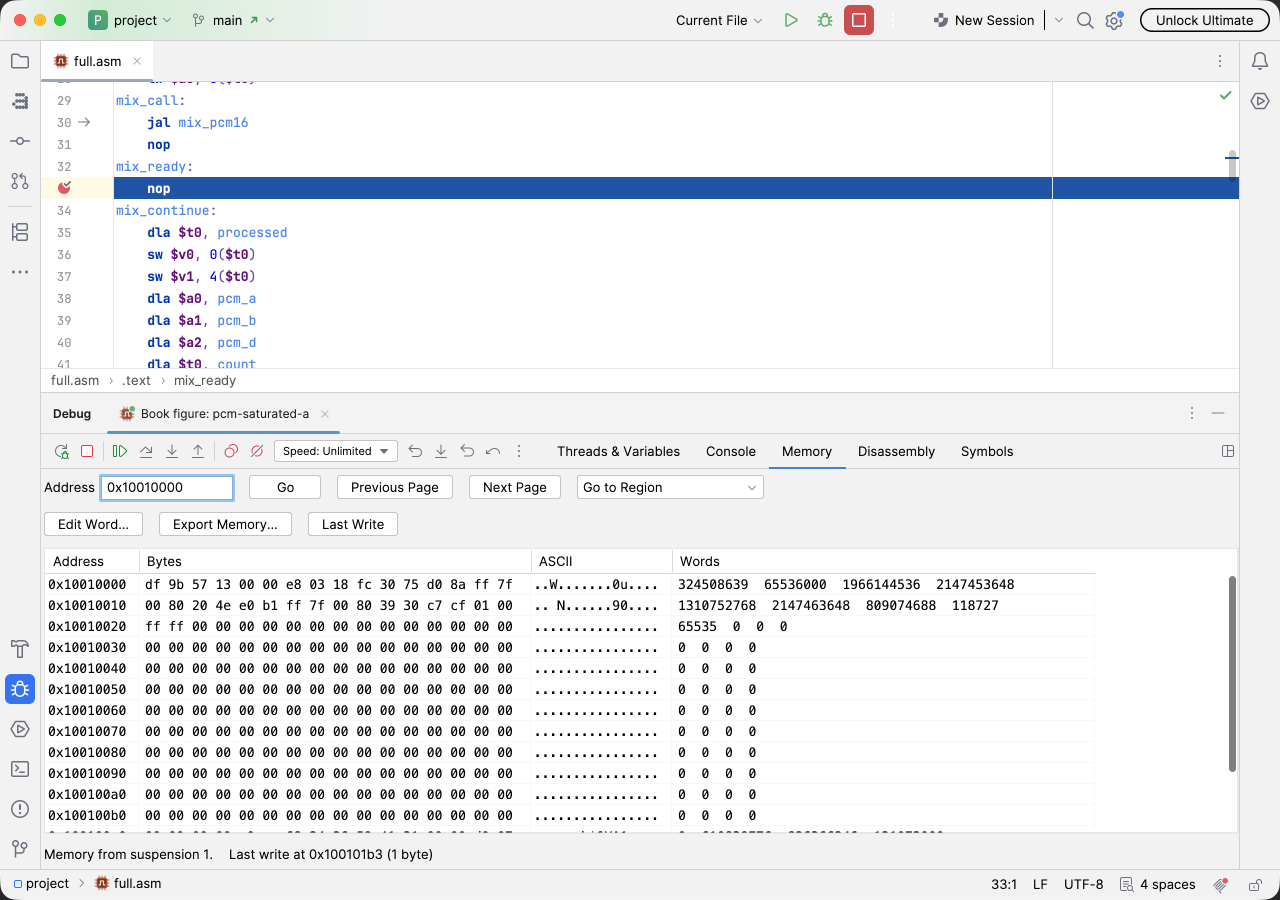
\includegraphics[width=0.84\linewidth,artifact,trim={\MARSpcmsaturatedaLeft{} \MARSpcmsaturatedaBottom{} \MARSpcmsaturatedaRight{} \MARSpcmsaturatedaTop{}},clip]{book/captures/020-pcm-mixing/f01/a.png}};
    \begin{scope}[shift={(a.south west)},x={($(a.south east)-(a.south west)$)},y={($(a.north west)-(a.south west)$)}]
      \draw[black,line width=0.7pt] (0.194672131,0.055555556) rectangle (0.997950820,0.638888889);
      \node[draw=black,fill=white,circle,inner sep=1.5pt,font=\footnotesize] at ($(0,0.638888889)+(-3mm,0)$) {3};
    \end{scope}
    \node[anchor=north west,inner sep=0,font=\small\bfseries] (b-title) at ([yshift=-1mm]a.south west) {Input B: signed halfwords};
    \node[anchor=north west,inner sep=0] (b) at ([yshift=-1mm]b-title.south west) {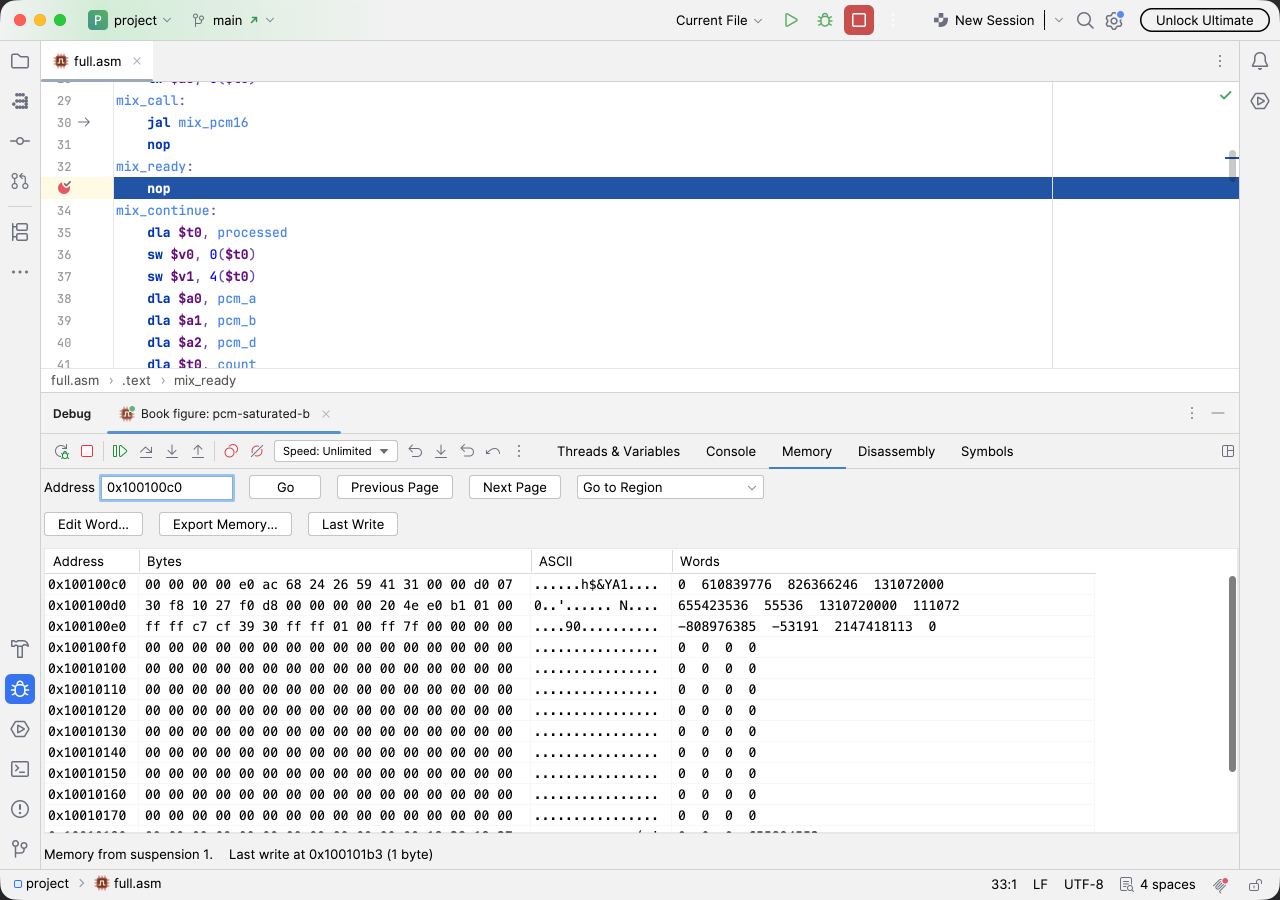
\includegraphics[width=0.84\linewidth,artifact,trim={\MARSpcmsaturatedbLeft{} \MARSpcmsaturatedbBottom{} \MARSpcmsaturatedbRight{} \MARSpcmsaturatedbTop{}},clip]{book/captures/020-pcm-mixing/f01/b.png}};
    \begin{scope}[shift={(b.south west)},x={($(b.south east)-(b.south west)$)},y={($(b.north west)-(b.south west)$)}]
      \draw[black,line width=0.7pt] (0.194672131,0.055555556) rectangle (0.997950820,0.638888889);
      \node[draw=black,fill=white,circle,inner sep=1.5pt,font=\footnotesize] at ($(0,0.638888889)+(-3mm,0)$) {4};
    \end{scope}
    \node[anchor=north west,inner sep=0,font=\small\bfseries] (saturated-title) at ([yshift=-1mm]b.south west) {Signed saturated samples};
    \node[anchor=north west,inner sep=0] (saturated) at ([yshift=-1mm]saturated-title.south west) {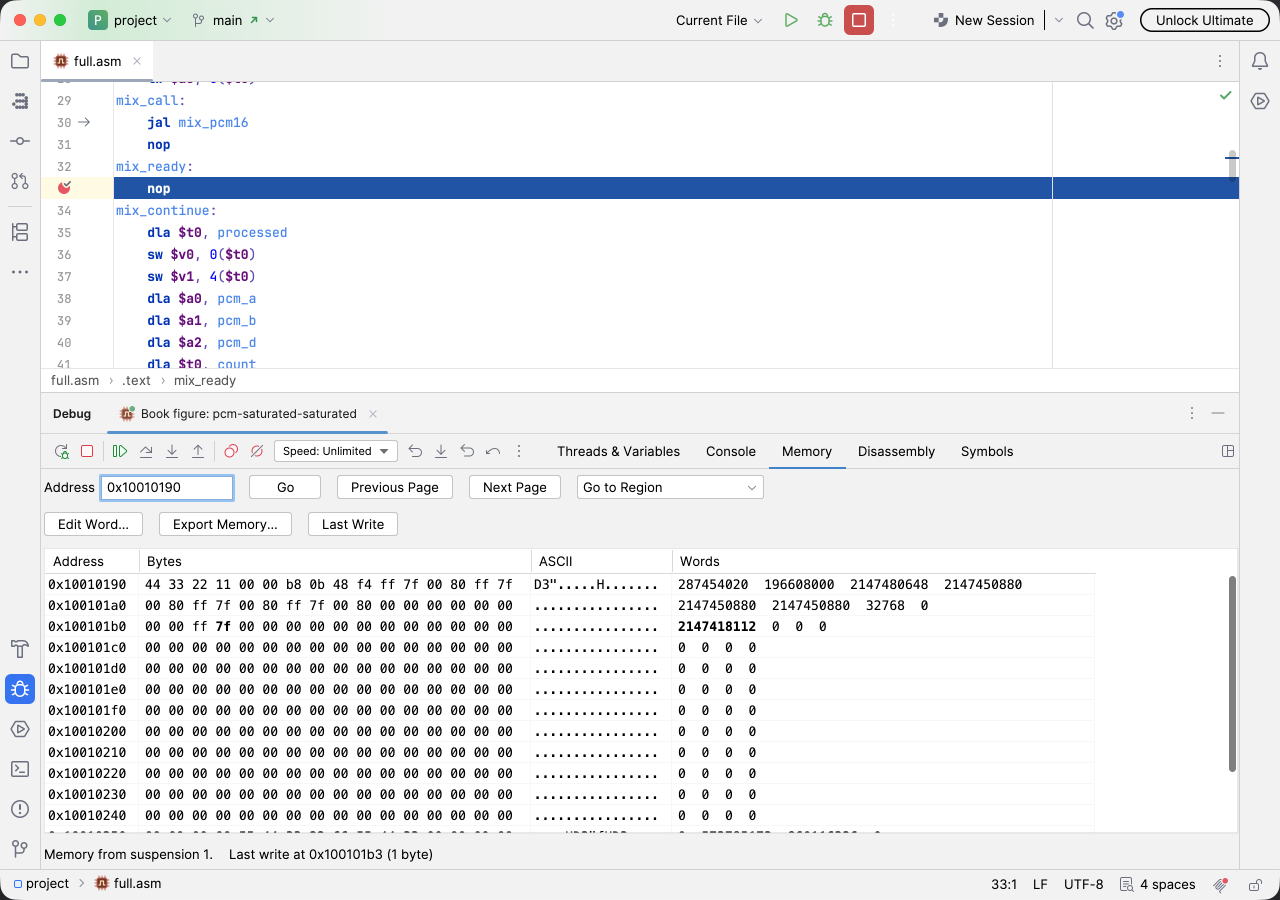
\includegraphics[width=0.84\linewidth,artifact,trim={\MARSpcmsaturatedsaturatedLeft{} \MARSpcmsaturatedsaturatedBottom{} \MARSpcmsaturatedsaturatedRight{} \MARSpcmsaturatedsaturatedTop{}},clip]{book/captures/020-pcm-mixing/f01/saturated.png}};
    \begin{scope}[shift={(saturated.south west)},x={($(saturated.south east)-(saturated.south west)$)},y={($(saturated.north west)-(saturated.south west)$)}]
      \draw[black,line width=0.7pt] (0.194672131,0.055555556) rectangle (0.997950820,0.638888889);
      \node[draw=black,fill=white,circle,inner sep=1.5pt,font=\footnotesize] at ($(0,0.638888889)+(-3mm,0)$) {5};
    \end{scope}
    \node[anchor=north west,inner sep=0,font=\small\bfseries] (caller-title) at ([yshift=-1mm]saturated.south west) {Count and saved caller results};
    \node[anchor=north west,inner sep=0] (caller) at ([yshift=-1mm]caller-title.south west) {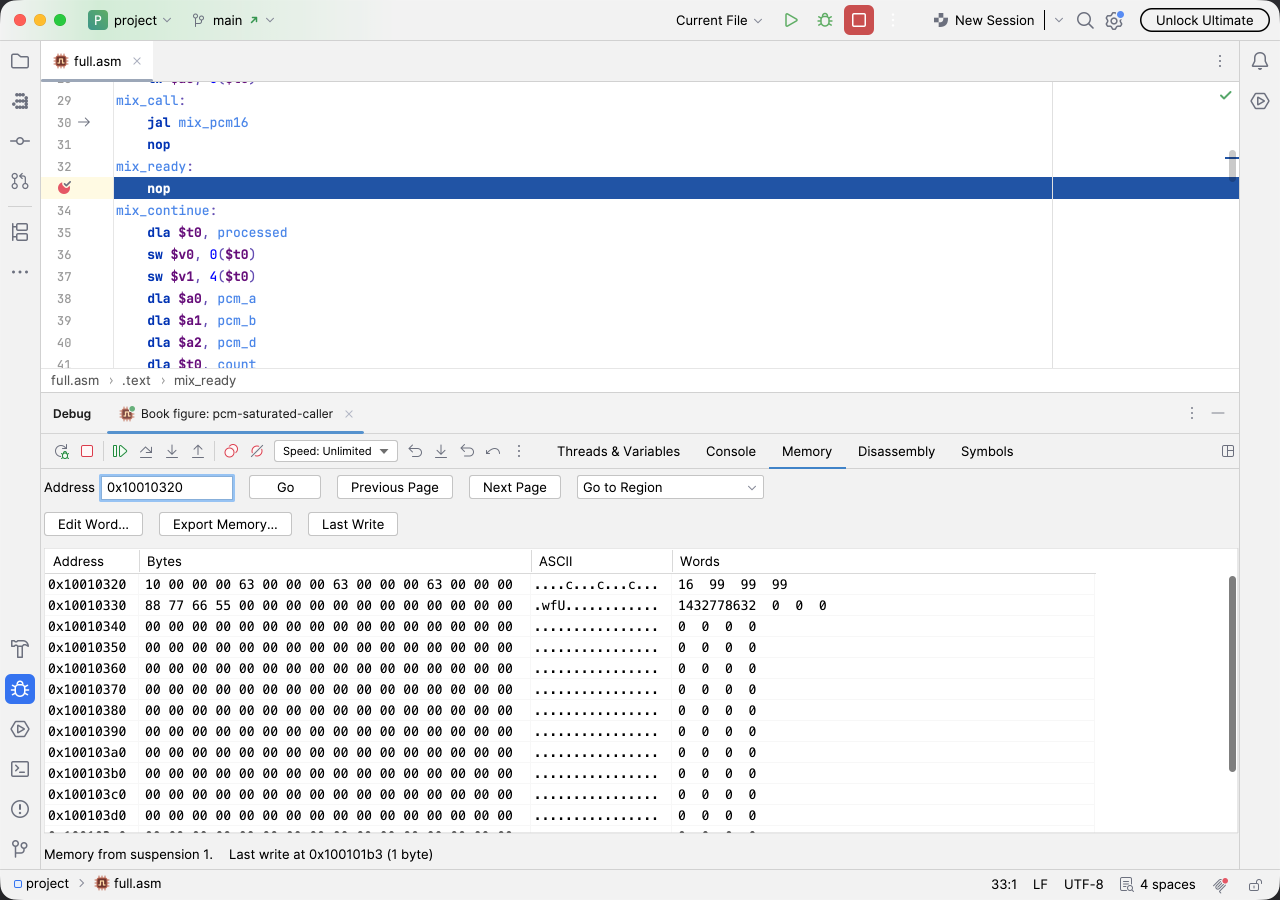
\includegraphics[width=0.84\linewidth,artifact,trim={\MARSpcmsaturatedcallerLeft{} \MARSpcmsaturatedcallerBottom{} \MARSpcmsaturatedcallerRight{} \MARSpcmsaturatedcallerTop{}},clip]{book/captures/020-pcm-mixing/f01/caller.png}};
    \begin{scope}[shift={(caller.south west)},x={($(caller.south east)-(caller.south west)$)},y={($(caller.north west)-(caller.south west)$)}]
      \draw[black,line width=0.7pt] (0.194672131,0.078431373) rectangle (0.997950820,0.490196078);
      \node[draw=black,fill=white,circle,inner sep=1.5pt,font=\footnotesize] at ($(0,0.490196078)+(-3mm,0)$) {6};
    \end{scope}
  \end{tikzpicture}
  \par\smallskip
  \begin{minipage}{\linewidth}
    \small
    \begin{enumerate}
      \setlength{\itemsep}{2pt}
            \setlength{\parsep}{0pt}
      \item The blue \texttt{nop} at \texttt{mix\_ready} follows the saturating mixer\textquotesingle s return. Output samples are ready. The caller has not yet copied either return register into its result words or invoked the wrapping comparison.
      \item \texttt{\$v0 = 16} counts processed samples; \texttt{\$v1 = 6} counts exact sums outside the signed-halfword range. The guided loop handles two eight-sample groups. An exact sum of 32767 or $-32768$ reaches an endpoint without counting as clipped.
      \item Input A starts at \texttt{0x10010004}, after its guard. Bytes \texttt{30 75} encode 30000 as \texttt{0x7530}; \texttt{d0 8a} encode $-30000$. Decode each low-byte-first pair as a signed halfword before forming the wider sum.
      \item Input B starts at \texttt{0x100100cc}. Its corresponding samples are 10000 (\texttt{10 27}) and $-10000$ (\texttt{f0 d8}). Their exact sums with the A values are 40000 and $-40000$, both outside the permitted output range.
      \item Saturated output starts at \texttt{0x10010194}. Sample 3 at \texttt{0x1001019a} is \texttt{ff 7f}, or 32767; sample 4 at \texttt{0x1001019c} is \texttt{00 80}, or $-32768$. The displayed bytes preserve the chosen endpoint rather than the overflowing sum\textquotesingle s low bits.
      \item The caller row contains count 16 followed by \texttt{processed}, \texttt{clipped} and \texttt{wrapped\_count}, all still 99. Bytes \texttt{63 00 00 00} encode each sentinel. Wrapping output is still untouched.
    \end{enumerate}
  \end{minipage}
  \caption{Saturation returns sixteen processed samples and six clipped sums before caller publication.}
  \label{capture:020-pcm-mixing-f01}
  \label{pcm-f01}
\end{figure}
\par
